\documentclass[conference]{IEEEtran}
\RequirePackage{cite}
\RequirePackage{amsmath,amssymb,amsfonts}
\RequirePackage{algorithmic}
\RequirePackage{graphicx}
\RequirePackage{textcomp}
\RequirePackage{xcolor}
\RequirePackage{hyperref}
\def\BibTeX{{\rm B\kern-.05em{\sc i\kern-.025em b}\kern-.08em
    T\kern-.1667em\lower.7ex\hbox{E}\kern-.125emX}}
\begin{document}
\title{EECS 106B Final Project Proposal}
\author{Andrew~Fearing, Neelay~Junnarkar,  Hamza~Kamran~Khawaja}
\maketitle


\begin{abstract} In this paper, we investigate algorithms that perform two-view and multi-view feature matching and reconstruction. The algorithms, namely the eight-point algorithm, the factorization algorithm, and the two-view triangulation as in \cite{ma2012invitation}. Data points from image sets depicting a city and house are used. The reconstructions after applying the algorithms are re-projected onto the original image/model and a re-projection error is calculated to evaluate performance. We found best performance with the two-view 8-point algorithm with a re-projection error of 4, while the four-view reconstruction had an error of 1624. In other words, least error was observed in two-view reconstruction, while most error was observed in multi-view reconstruction.
\end{abstract}


\section{About Us}
Neelay is a 4th year undergraduate in EECS, and has taken courses such as EE 128, 221A/222, and (of course) EECS 106A. His interests are primarily related to control and motion planning.

Andrew is a 4th year undergraduate in EECS. He has taken EE 120, EE C128, and EECS C106A. His interests in robotics are in micro-scale mobile robots.
\section{Research Question}
Can we control a boat so that it keeps its lane? Autonomously navigate a canal.
\section{Motivation}
Boat stuck.
\begin{figure}
    \centering
    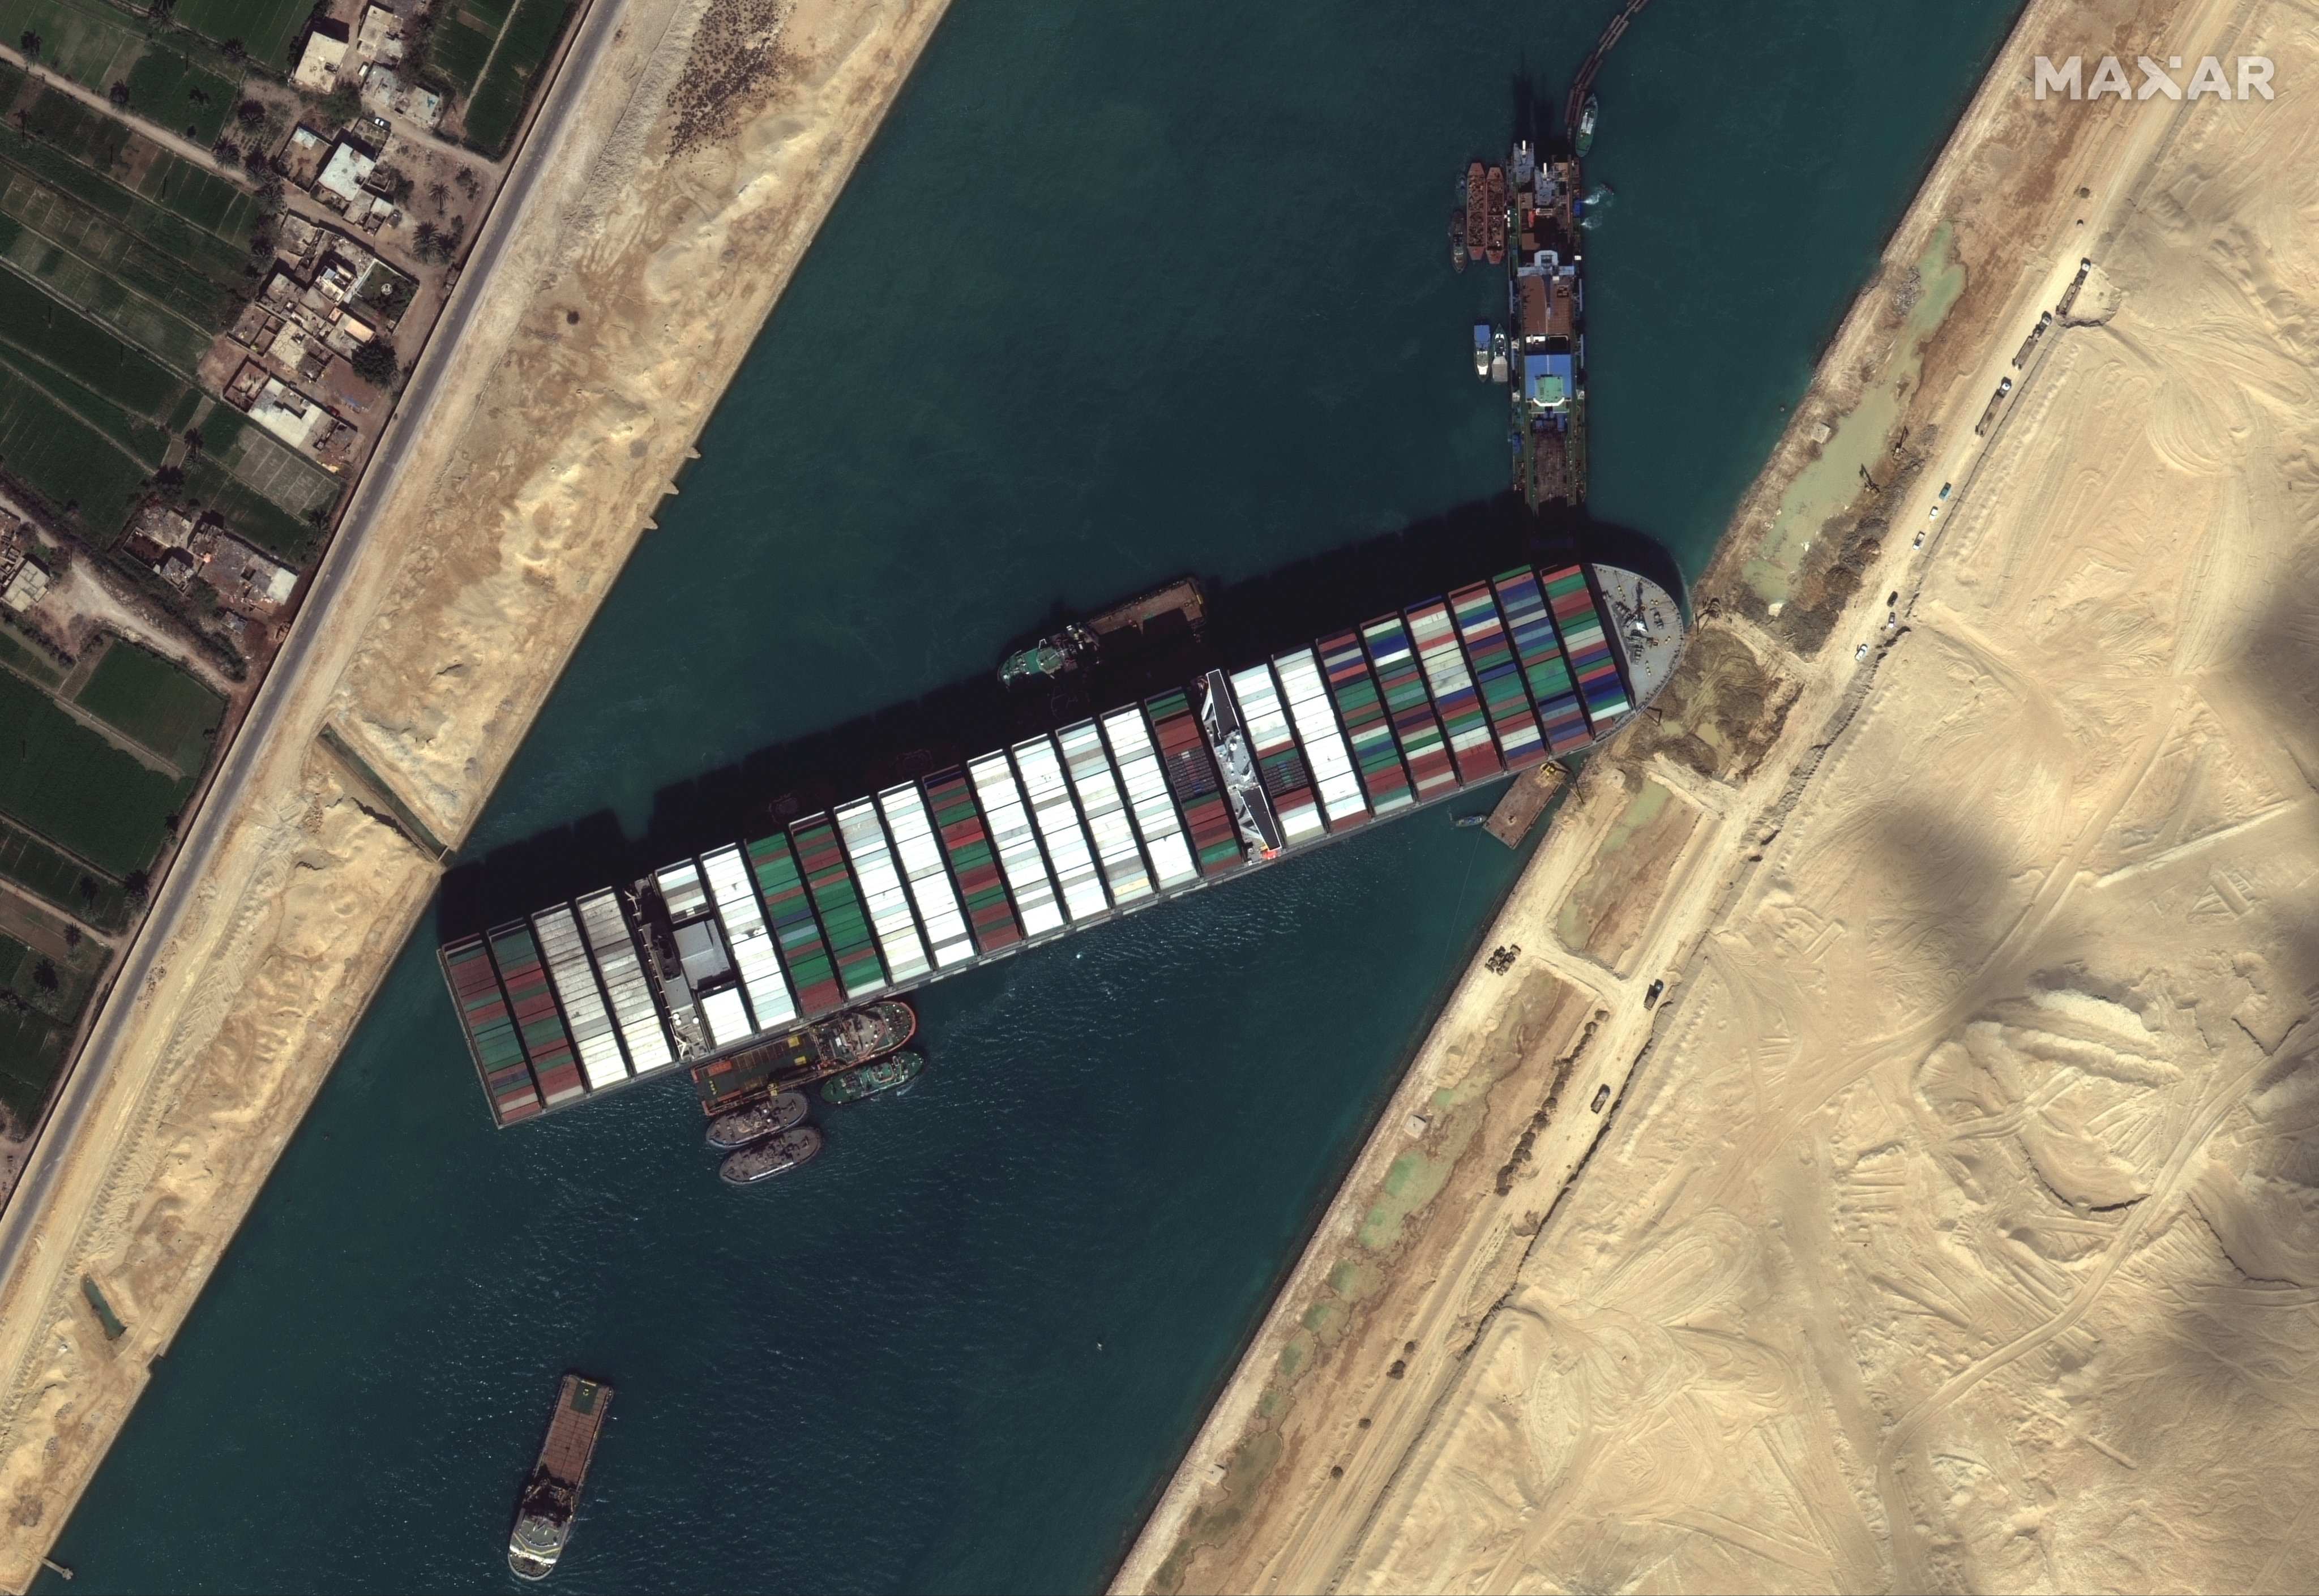
\includegraphics{documents/proposal/Suez_Canal_blocked_by_Ever_Given_March_27_2021.jpg}
    \caption{Boat stuck\label{fig:boat_stuck}}
\end{figure}
Control and safety of automobiles is an area of intense research focus. We want to tackle a 
\section{Proposed Methodology}

\section{Related Work}

\section{Experimental Plan}


\bibliographystyle{IEEEtran}
\bibliography{../lit_review/refs.bib}
\end{document}